% Fig. 1 -- USGLoc overview (standalone TikZ -> vector PDF).
% Compile standalone: pdflatex fig1_overview.tex
% In the paper: \resizebox{\textwidth}{!}{\input{figures/fig1_overview}}
%
% Design (after the STDLoc / UGS-Loc / GS-CPR / SplatHLoc figure study):
%  * slim grey OFFLINE strip (evidential mapping) on the left;
%  * Band A: the online pose flow (query -> matching -> hypotheses ->
%    refinement -> calibrated posterior);
%  * Band B: the EVIDENCE channel in gold underneath, injected upward into
%    Band A at four points (gate, correspondence gate, per-pixel weight,
%    temperature) -- the paper's thesis as the figure's macro-structure;
%  * every arrow carries an artifact glyph and a math symbol from the text;
%  * two accent colors only: gold = evidence, blue = pose distributions.
\documentclass[tikz,border=3pt]{standalone}
\usepackage{amsmath,amssymb,bm}
\usepackage{graphicx}
\usetikzlibrary{positioning,arrows.meta,backgrounds,fit,calc,shadings}

\definecolor{ink}{HTML}{273746}
\definecolor{uLow}{HTML}{1B9E77}
\definecolor{uMid}{HTML}{E6AB02}
\definecolor{uHigh}{HTML}{D95F02}
\definecolor{coarseBg}{HTML}{EAF2FB}
\definecolor{coarseLn}{HTML}{9DC3EC}
\definecolor{fineBg}{HTML}{FDF1E6}
\definecolor{fineLn}{HTML}{F0C28E}
\definecolor{encBg}{HTML}{EEF6EE}
\definecolor{encLn}{HTML}{B7D8B7}
\definecolor{outBg}{HTML}{FFF3D6}
\definecolor{outLn}{HTML}{D9A300}
\definecolor{poseC}{HTML}{2E6FAC}

\begin{document}
\begin{tikzpicture}[
  font=\footnotesize\color{ink},
  >={Stealth[length=2mm]},
  mod/.style={draw=ink!75, fill=white, rounded corners=2pt, align=center,
              minimum height=10mm, inner sep=2.5pt, line width=0.5pt},
  flow/.style={->, line width=0.7pt, draw=ink!80},
  evflow/.style={->, line width=1.0pt, draw=outLn},
  inject/.style={->, line width=1.0pt, draw=outLn, dashed},
  sym/.style={font=\scriptsize\color{ink}, inner sep=1.5pt, fill=white,
              fill opacity=0.85, text opacity=1},
  sub/.style={font=\scriptsize\color{ink!75}, align=center},
  panlab/.style={font=\scriptsize\bfseries\color{ink!80}}
]

% ============================ OFFLINE STRIP =================================
% mapping frames: three real training views
\foreach \i/\dx/\dy in {2/0.16/0.16, 1/0.08/0.08, 0/0/0}{
  \node[inner sep=0pt, draw=ink!60, line width=0.35pt]
    at (1.15+\dx, 1.42+\dy) {\includegraphics[width=10mm]{fig1_blocks/mapframe\i.png}};
}
\node[sub, anchor=north] at (1.15, 0.92) {mapping frames};
\draw[flow] (1.15, 0.72) -- (1.15, 0.12);
\node[mod, text width=23mm, font=\scriptsize\color{ink}] (edlhead) at (1.15,-0.42)
  {semantic 3DGS\\ + EDL head (3)};
\draw[flow] (1.15,-0.98) -- node[sym, right=0mm] {$(\mathbf{b},u)$} (1.15,-1.22);
% evidential map: splats colored by vacuity
% the real map, rendered from a free camera: Gaussians, not a schematic
\node[inner sep=0pt, draw=ink!60, line width=0.35pt] (map3d) at (1.15,-2.00)
  {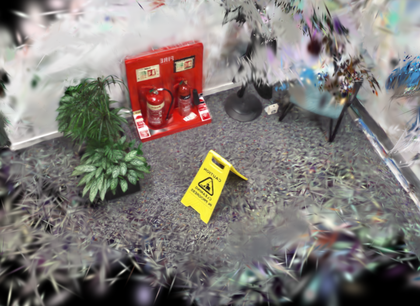
\includegraphics[width=20mm]{fig1_blocks/map3d.png}};
% vacuity key, so the colour channel carried below means something
\foreach \i/\c in {0/uLow, 1/uMid, 2/uHigh}{
  \shade[inner color=\c!25, outer color=\c!85] (0.42+0.26*\i, -3.00) circle (0.9mm);
}
\node[sub, anchor=west, font=\tiny\color{ink!75}] at (1.08,-3.00) {$u$: low$\to$high};
\node[sub, anchor=north, text width=30mm] at (1.15,-3.18)
  {evidential map $\mathcal{M}{=}\{\mathcal{G}_i\}$\\[-0.4mm]
   {\tiny $\mathcal{G}_i{=}(\bm\mu_i,\bm\Sigma_i,f_i,\mathbf{p}_i,\tilde u_i)$}};

% ============================== BAND A ======================================
% query
\node[inner sep=0pt, draw=ink!70, line width=0.5pt] (qimg) at (3.92, 1.01)
  {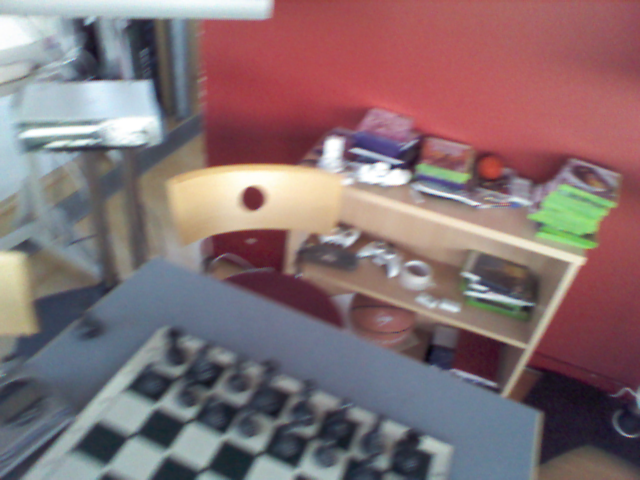
\includegraphics[width=11.5mm]{fig4/a_query.png}};
\node[sub, anchor=north] at (3.92, 0.55) {query $I_q$};

% evidential encoding
\node[mod, text width=25mm] (enc) at (6.05, 1.0)
  {Evidential\\encoding (III-B)\\{\scriptsize $\mathcal{Q}_j{=}(\mathbf{x},a,f^q,\mathbf{p}^q,u^q)$}};
\draw[flow] (4.5, 1.0) -- (enc.west);

% gated matching, with match-line glyph showing gating
\node[mod, text width=24mm, minimum height=13mm] (match) at (9.35, 1.0)
  {Vacuity-gated\\matching (III-C)};
\draw[flow] (enc.east) -- node[sym, above=0mm] {$d^q_j$} (match.west);
% match glyph below the box: two frames, kept (green) and gated-out (orange) matches
\begin{scope}[shift={(8.55, 0.28)}]
  \draw[ink!55, line width=0.4pt] (0,0) rectangle +(0.5,0.36);
  \draw[ink!55, line width=0.4pt] (1.1,0) rectangle +(0.5,0.36);
  \draw[uLow, line width=0.5pt]  (0.5,0.28) -- (1.1,0.30);
  \draw[uLow, line width=0.5pt]  (0.5,0.16) -- (1.1,0.12);
  \draw[uHigh, line width=0.5pt, dash pattern=on 1pt off 1pt] (0.5,0.05) -- (1.1,0.22);
\end{scope}

% top-k hypotheses: three fading camera frusta
\begin{scope}[shift={(12.15, 0.72)}]
  \foreach \dx/\op in {0/0.9, 0.42/0.55, 0.84/0.3}{
    \begin{scope}[shift={(\dx,0)}, opacity=\op]
      \fill[poseC!25] (0,0.66) -- (0,0.10) -- (0.5,0.38) -- cycle;
      \draw[poseC, line width=0.6pt] (0,0.66) -- (0,0.10) -- (0.5,0.38) -- cycle;
    \end{scope}
  }
\end{scope}
\node[sub, anchor=north, text width=24mm] (hyplab) at (12.85, 0.62)
  {top-$k$ hypotheses\\$\{(T^0_k,\tilde\pi_k)\}$};
\draw[flow] (match.east) -- node[sym, above=0mm] {$s_{ij}$ (6)} (12.0, 1.0);

% ---- row 2 (correction + fine + pose head), shifted under row 1 ----------
\node[mod, text width=24mm, minimum height=13mm] (corr) at (3.50, -5.80)
  {Matching\\correction (III-D)\\{\scriptsize PnP on gated matches (8)}};
\node[mod, text width=26mm, minimum height=13mm] (refine) at (6.75, -5.80)
  {Vacuity-weighted\\refinement (III-E)\\{\scriptsize $E(\bm{\xi})$ (10)}};
\node[inner sep=0pt, draw=ink!55, line width=0.4pt] (wimg) at (6.75,-7.15)
  {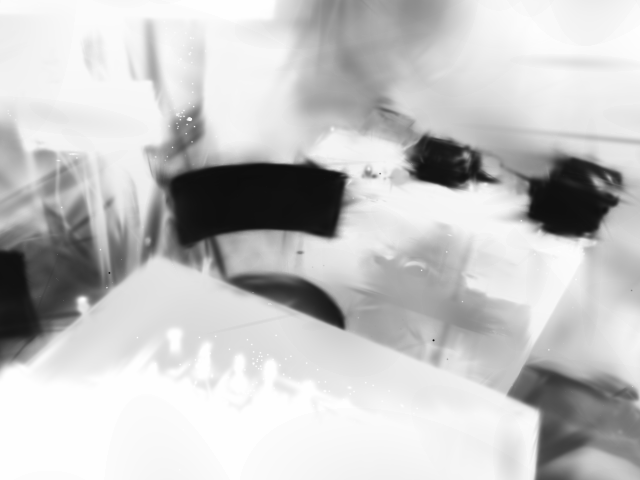
\includegraphics[width=12mm]{fig4/a_weight.png}};
\node[sub, anchor=north] at (6.75,-7.58) {per-pixel weight $w$};
\draw[flow] (corr.east) -- node[sym, above=0mm] {$T'_k$} (refine.west);

% ---- calibrated pose head ----
\node[mod, text width=21mm] (lap) at (10.15, -5.80)
  {Laplace cov.\ (11)\\{\scriptsize $\bm{\Sigma}_{\bm{\xi},k}\!\leftarrow\!\tau\hat\sigma^2(J^{\!\top}\!WJ)^{-1}$}};
\draw[flow] (refine.east) -- node[sym, above=0mm] {$\bm{\xi}^\star_k$} (lap.west);
% GMM glyph: overlapping covariance ellipses
\begin{scope}[shift={(12.55, -5.98)}]
  \draw[poseC!85, line width=0.6pt, rotate around={18:(0.32,0.28)}]
    (0.32,0.28) ellipse (4.6mm and 2.4mm);
  \draw[poseC!85, line width=0.6pt, rotate around={-12:(0.95,0.46)}]
    (0.95,0.46) ellipse (3.2mm and 1.8mm);
  \fill[poseC] (0.32,0.28) circle (0.5pt);
  \fill[poseC] (0.95,0.46) circle (0.5pt);
\end{scope}
\node[sub, anchor=north, text width=26mm] at (13.20, -6.25)
  {$p(T|I_q,\mathcal{M})$ (12)\\condense $\rightarrow$ EKF};
\draw[flow] (lap.east) -- (11.95, -5.80);

% ---- the serpentine turn: row 1 ends, row 2 begins -----------------------
\draw[flow] (13.85, 1.0) -- (14.75, 1.0) -- (14.75, -4.12)
            -- (1.30, -4.12) -- (1.30, -5.80) -- (corr.west);


% ============================== BAND B ======================================
% opinion simplex glyph
\begin{scope}[shift={(5.55,-2.65)}]
  \draw[outLn, line width=0.6pt] (0,0) -- (1.0,0) -- (0.5,0.8) -- cycle;
  \fill[outLn!45] (0.42,0.30) circle (1.6mm);
  \node[sub, anchor=north] at (0.5,-0.08) {opinion $(\mathbf{b},u)$};
\end{scope}
% DST fusion glyph: two small simplexes -> one
\begin{scope}[shift={(8.55,-2.45)}]
  \draw[outLn!70, line width=0.5pt] (0,0.12) -- (0.44,0.12) -- (0.22,0.48) -- cycle;
  \draw[outLn!70, line width=0.5pt] (0,-0.42) -- (0.44,-0.42) -- (0.22,-0.06) -- cycle;
  \node[font=\scriptsize\color{outLn}] at (0.68,-0.02) {$\oplus$};
  \draw[outLn, line width=0.6pt] (0.9,-0.28) -- (1.5,-0.28) -- (1.2,0.22) -- cycle;
  \node[sub, anchor=north, text width=24mm] at (0.26,-0.56)
    {conflict-aware fusion (4)\\[-0.3mm]{\tiny $\tilde{u}{=}\min(1,u{+}\bar\eta)$}};
\end{scope}
% vacuity heatmap glyph U_r
\node[inner sep=0pt, draw=ink!55, line width=0.4pt] (urimg) at (10.95,-2.34)
  {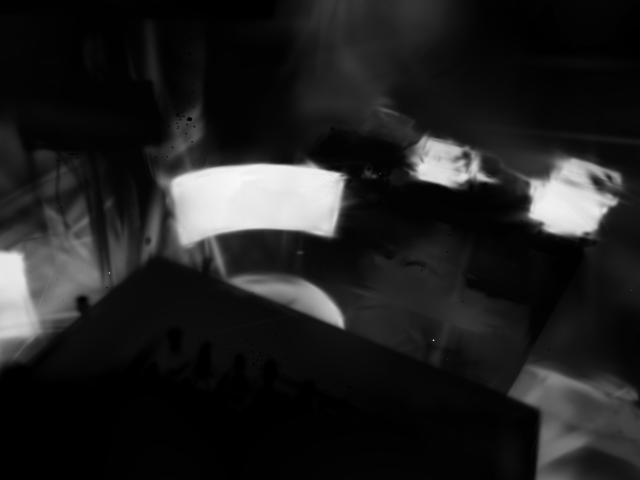
\includegraphics[width=12mm]{fig4/a_vacuity.png}};
\node[sub, anchor=north] at (11.05,-2.90) {rendered $U_r$ (9)};
% temperature chip
\node[mod, draw=outLn, text width=16mm, font=\scriptsize\color{ink}] (temp) at (13.35,-2.45)
  {temperature $\tau$\\(held-out fit)};

% the gold evidence rail
\draw[evflow] (2.1,-2.1) -- node[sym, above=0mm] {$u$} (5.45,-2.35);
\draw[evflow] (6.75,-2.35) -- (8.4,-2.5);
\draw[evflow] (9.95,-2.34) -- node[sym, above=0.6mm, pos=0.45] {$\tilde{u}_i$ per splat} (urimg.west);
\draw[evflow] (urimg.east) -- (temp.west);

% injections: UP into row 1, DOWN into row 2 -- one channel, both bands
\draw[inject] (9.35,-1.95) -- node[sym, right=0.2mm]
  {gate $e^{-\lambda_u(\tilde{u}^G_i+u^q_j)}$} (match.south);
\draw[inject] (10.25,-3.60) -- node[sym, left=0.2mm, pos=0.42, fill=white, inner sep=1pt]
  {$\bar U_r{\le}u_{\max}$} (corr.north);
\draw[inject] (11.65,-3.60) -- node[sym, right=0.2mm, pos=0.42, fill=white, inner sep=1pt]
  {$w{=}e^{-\gamma U_r}$} (refine.north);
\draw[inject] (temp.south) -- node[sym, right=0.2mm] {$\tau$} (lap.north);

% ======================= PANELS (background layer) ==========================
\begin{scope}[on background layer]
  % offline strip
  \node[fill=ink!5, draw=ink!35, dashed, rounded corners=3pt, inner sep=2.6mm,
        fit={(edlhead) (map3d) (-0.20,2.05) (2.55,-3.95)}] (offpan) {};
  % coarse panel
  \node[fill=coarseBg, draw=coarseLn, rounded corners=3pt, inner sep=2.8mm,
        fit={(enc) (match) (hyplab) (13.9,0.2)}] (cpan) {};
  % fine panel
  \node[fill=fineBg, draw=fineLn, rounded corners=3pt, inner sep=2.8mm,
        fit={(corr) (refine) (wimg) (6.75,-7.75)}] (fpan) {};
  % calibrated pose head panel
  \node[fill=poseC!8, draw=poseC!60, rounded corners=3pt, inner sep=2.8mm,
        fit={(lap) (14.6,-6.45) (14.6,-5.25)}] (ppan) {};
  % evidence band
  \node[fill=outBg, draw=outLn!70, rounded corners=3pt, inner sep=2.8mm,
        fit={(5.45,-1.8) (temp) (urimg) (14.3,-3.42) (5.45,-3.42)}] (epan) {};
\end{scope}
\node[panlab, anchor=south west] at (offpan.north west)
  {Offline: evidential mapping (III-A)};
\node[panlab, anchor=south west] at (cpan.north west) {Coarse (IV-B,C)};
\node[panlab, anchor=south west] at (fpan.north west) {Correction + fine (IV-D,E)};
\node[panlab, anchor=south west, color=poseC] at (ppan.north west)
  {Calibrated pose posterior};
\node[panlab, anchor=south west, color=outLn!80!ink] at (epan.north west)
  {One evidential channel: created once, never dropped};

% map feeds the online flow
\draw[flow] (2.18,-0.42) -- node[sym, above=0.4mm, pos=0.62] {$\mathcal{M}$}
  (2.95,-0.42) -- (8.4,-0.42) -- (match.south west);

\end{tikzpicture}
\end{document}
